\problemname{Craters}
General Warren Pierce has a bit of a problem.  He's in charge of a new type
of drone-delivered explosive and they've been testing it out in the Nevada
desert, far enough from any population center to avoid civilian casualties
and prying eyes.
Unfortunately word has gotten out about these experiments and now there's the
possibility of careless on-lookers, nefarious spies, or even worse --- nosy
reporters!
To keep them away from the testing area, Warren wants to erect a single fence
surrounding all of the circular craters produced by the explosions.
However, due to various funding cuts (to
support tax cuts for the you-know-who) he can't just put up miles and miles of
fencing like in the good old days. He figures that if he can keep people at
least $10$ yards away from any crater he'll be okay, but he's unsure of how much
fencing to request.  Given the locations and sizes of the craters, can you
help the General determine the minimum amount of fencing he needs?  An
example with three craters (specified in Sample Input 1) is shown below.

\begin{figure}[!h]
\centering
  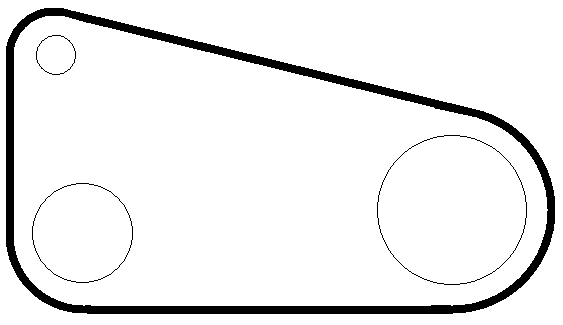
\includegraphics{crater}
  \vspace{-3pt}%
  \caption{Three craters with a fence around them.}
  \label{craters_1}
\end{figure}

\section*{Input}
The first line of input contains a single positive integer $n$ $(n \leq 200)$,
the number of craters.  After this are $n$ lines specifying the location and
radius of each crater.  Each of these lines contains 3 integers $x$ $y$ $r$,
where $x$ and $y$ specify the location of a crater $(|x,y| \leq 10\,000)$ and $r$
is its radius ($0 < r \leq 5\,000$).  All units are in yards.


\section*{Output}
Display the minimum amount of fencing (in yards) needed to cordon off the
craters, with an absolute or relative error of at most $10^{-6}$.
